\documentclass[a4paper,11pt,oneside]{article}
\usepackage[a4paper,margin=3cm]{geometry}
\pagestyle{headings}

\usepackage[T1]{fontenc}
\usepackage[utf8]{inputenc}
\usepackage[australian]{babel}
\usepackage{fourier}
\usepackage{pdflscape}
\usepackage{titlesec}

\usepackage{microtype}
\usepackage{indentfirst}
\usepackage{enumitem}

\usepackage{quoting}
\usepackage{caption}

\usepackage{booktabs}
\usepackage{tabularx}
\usepackage{verbatim}

\usepackage{graphicx}
\usepackage{listings}
\usepackage{fancyvrb}
\usepackage{xcolor}

\usepackage{ulem}

\usepackage{hyperref}


\newcommand{\email}[1]{\href{mailto:#1}{\texttt{#1}}}
\newenvironment{bottompar}{\par\vspace*{\fill}}{\clearpage}
\renewcommand\arraystretch{1.3}

\newcommand\m[1]{
	\centering
	\renewcommand\arraystretch{1.1}
	\begin{tabular}{@{}c@{}}#1\end{tabular}
}
\newcommand{\centered}[1]{\begin{tabular}{c} #1 \end{tabular}}

\renewcommand{\tabularxcolumn}[1]{m{#1}}
\newcolumntype{L}{>{\raggedright}X}
\newcolumntype{C}{>{\centering\arraybackslash}X}

\captionsetup{format=hang,labelfont=it,font=small, skip=5pt}
\quotingsetup{font=small}
\hypersetup{
	colorlinks=true,
	linkcolor=black,
	urlcolor=blue,
	citecolor=magenta,
	filecolor=magenta,
}
\renewcommand{\ULdepth}{1.8pt}

\graphicspath{{imgs/}}

\begin{document}

	\author{}
	\title{\textbf{Introduction to Databases - Final Project}}
	\date{5 February 2021}
	\maketitle

	\tableofcontents
	\newcommand{\sectionbreak}{\clearpage}

	\section{Conceptual Design}

\subsection{Requirements}

	Objective of the database is to store the timetable of public transportation service within a single region. Following is a description of the information that is relevant and as such is represented in the database. \medskip
	
	A \textbf{trip} (identified by a code) consist of an ordered sequence of \textbf{stops}, each with arrival and departure times. The first stop of a trip does not have an arrival time, and the last one does not have a departure time. It \textbf{runs} on a defined period of the year, normally on specific days of the week and optionally on other dates, in which it can be exceptional or suppressed. \textit{For example, a trip could run within 14/09/2020 (included) and 26/06/2021 (excluded) from Monday to Friday, but not if the day is a public holiday. Another could run in the same dates range on Sunday, and also if the day is a public holiday.}
	
	A trip is part of a \textbf{line} and is conducted by a driver of a specific \textbf{company}, of which the name and the headquarter city are of interest. Of a line, the short code \textit{(e.g. 10A)}, a brief description \textit{(e.g. Hospital-City Centre-Hospital)}, the color, the city in which it originates and the type of vehicle \textit{(e.g. bus or train)} are of interest. The short code is unique only within a single city.
	
	A stop is instead characterized by the name, the \textbf{city} and the coordinates. When considering bus or train stations, the stopping point should also contain the platform name. The stop name should be memorized in different languages \textit{(e.g. in Italian and German)}. It is also the case that at least one translation is present, and if there is more than one translation, then all stop names are translated in all the possible languages.

\subsection{ER Schema}

	See Figure \ref{img:diagram} on next page.	

	\begin{landscape}
		\begin{figure}[htb]
			\thispagestyle{plain}
			\centering
			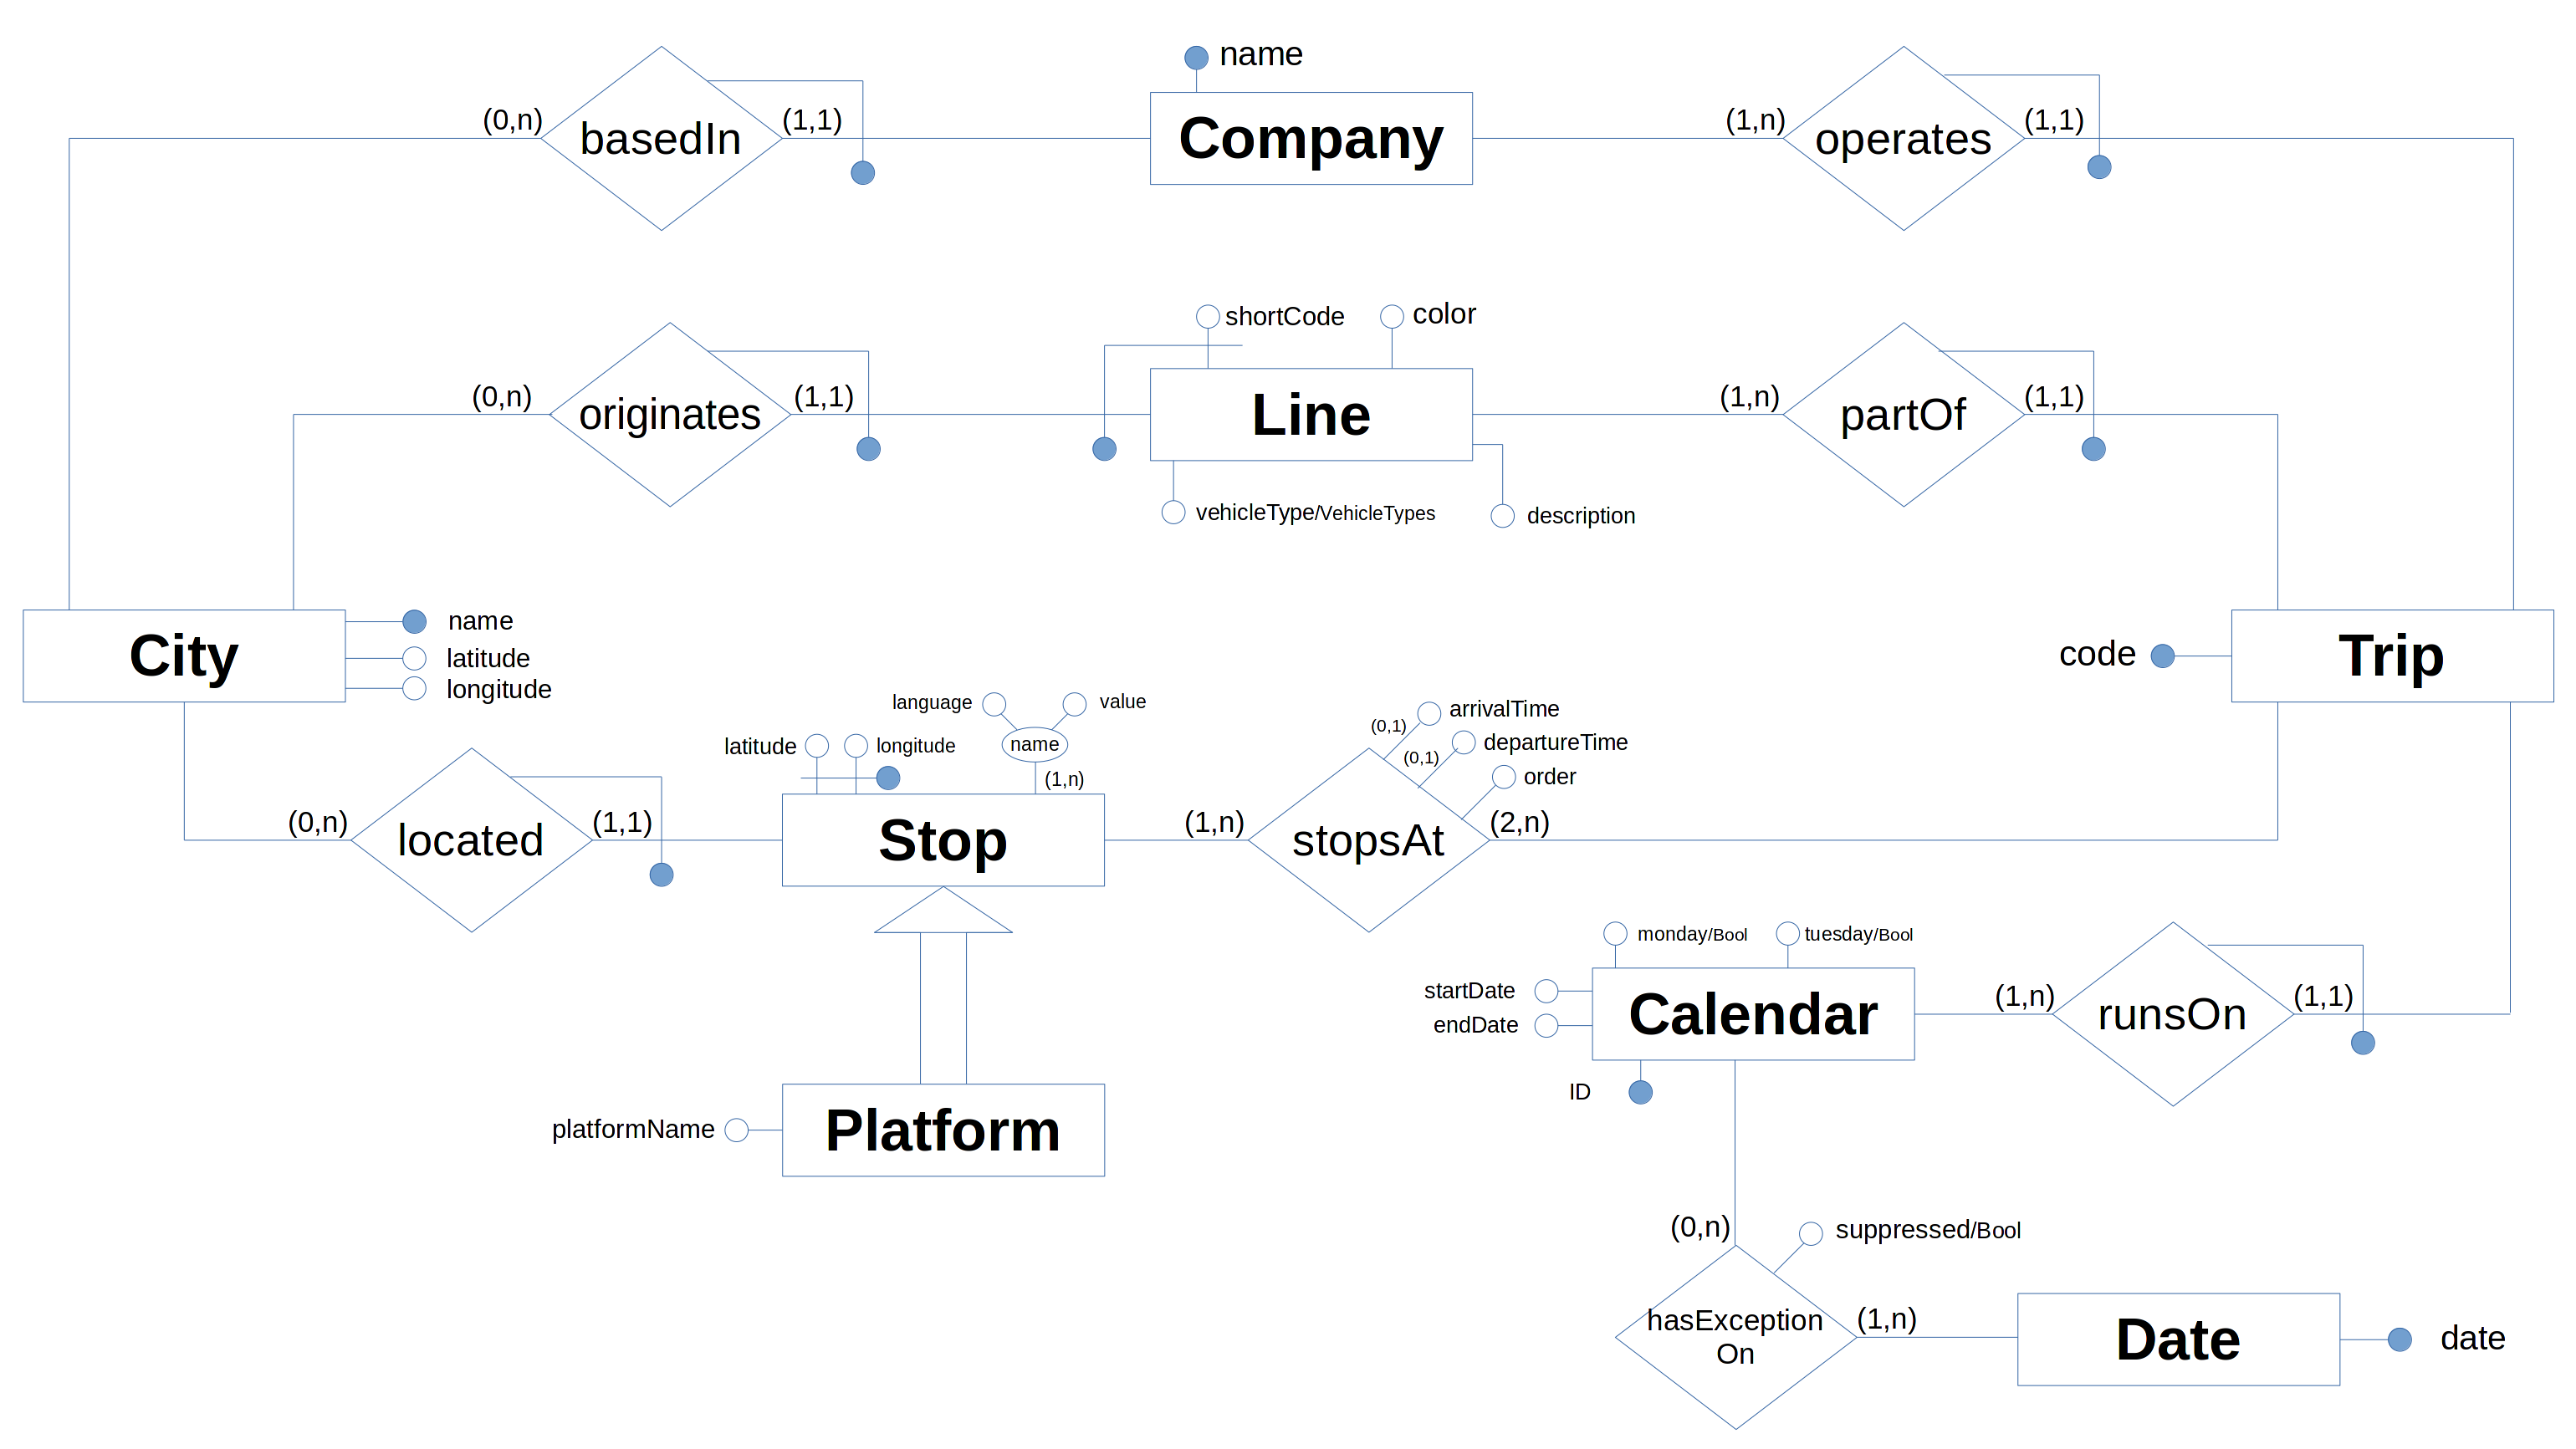
\includegraphics[height=\textheight]{imgs/diagram}
			\caption{ER Schema \\ {\footnotesize \textit{Note: not all attributes have been indicated in the schema. Please check the \hyperref[sec:dictionary]{data dictionary} for a complete overview}}}\label{img:diagram}
		\end{figure}
	\end{landscape}
	



\subsection{Glossary}

	\begin{table}[htb]
		\centering
		\begin{tabularx}{\columnwidth}{|c|C|}
			\hline
			\textbf{Term} & \textbf{Description} \\
			\hline
			\textbf{Stop} & Physical location in which passengers get on or off a vehicle  \\ \hline
			\textbf{Station} & Large stop consisting of many platform, where more than one vehicle can board passengers at the same time  \\ \hline
			\textbf{Platform} & Single stopping point inside a Station. It is represented by a number \\ \hline
			\textbf{Line} & Group of trips that follow the same route and is identified to the public with the same number or code  \\ \hline
			\textbf{Trip} & Ordered sequence of two or more stops, each with arrival and departure times \\ \hline
			\textbf{Calendar} & Defines when a trip runs in terms of date ranges and days of the week \\ \hline
			\textbf{Company} & Firm that is responsible of operating a trip \\
			\hline
		\end{tabularx}
		\caption{Glossary}\label{tbl:glossary}
	\end{table}

	\subsection{Data Dictionary}
	\label{sec:dictionary}

	\subsubsection{External Constraints}

	For completeness, all possible constraints have ben enlisted. Note that some of them can not be enforced at database level, either due to the lack functionalities of the DBMS or for the high complexity that they have. In particular, only constraints 1-4 will be checked by the DBMS.
	
	\begin{enumerate}
		\item For each tuple in the entity \texttt{Calendar}, the attribute \textit{endDate} must encode a date strictly greater than \textit{startDate}.
		
		\item For each tuple in the relationship \texttt{stopsAt}, the attribute \textit{departureTime} must encode a time greater or equal than \textit{arrivalTime}.
		
		\item In the relationship \texttt{stopsAt}, for the first stop of each \texttt{trip} (with \textit{order=1}), the attribute \textit{arrivalTime} must be omitted and \textit{departureTime} must be specified. For the last stop (with maximal \textit{order} for the trip), the attribute \textit{arrivalTime} must be specified and \textit{departureTime} must be omitted. For all the other stops, both attributes must be present.
		
		\item In the relationship \texttt{stopsAt}, the attribute \textit{order} must be equal to \texttt{1} for the first stop of a trip, and should be incremented by one for subsequent stops.
		
		\item In the relationship \texttt{stopsAt}, for every pair of tuples \textit{T1} and \textit{T2} within the same trip, if \textit{T1[order] < T2[order]}, then \textit{T1[departureTime] < T2[arrivalTime]}

		\item For a \texttt{Calendar}, the exceptional dates defined through the \texttt{hasExceptionOn} relationship must be in between \textit{startDate} and \textit{endDate}. Moreover, if \textit{suppressed=True} then the corresponding day of week has value \textit{True} (that is, trips will be exceptionally suppressed on that day, since normally on that day of week they do run). On the opposite, if \textit{suppressed=False} then the corresponding day of week has value \textit{False} (that is, trips will exceptionally run on that day, since normally they do not run on that day of week).
	\end{enumerate} 

	\subsubsection{Entities}
	
	See tables \ref{tbl:entites} and \ref{tbl:relationships}.
	
	\begin{table}[h!]
		\centering
		\begin{tabularx}{\columnwidth}{|c|C|C|c|}
			\hline
			\textbf{Entity} & \textbf{Description} & \textbf{Attributes} & \textbf{Identifiers} \\
			\hline
			\textbf{Calendar} & List of dates for which a trip runs. It defines a date range, with start and end date, together with the days of week in which the trip normally runs.
			
			Each day of week is a boolean value, so that if the value is \texttt{true} the trip runs on that day, otherwise it does not. & ID, startDate, endDate, monday, tuesday, wednesday, thursday, friday, saturday, sunday & \{ID\} \\ \hline
			\textbf{City} & Represents a city within the region of interest. & name, latitude, longitude & \{name\} \\ \hline
			\textbf{Company} & Transportation company responsible for running a set of trips & name & \{name\} \\ \hline
			\textbf{Date} & Specific date for which there is an exception (the corresponding trips are either suppressed or run exceptionally)& date & \{date\} \\ \hline
			\textbf{Line} & A public transportation line, ran by a specific kind of vehicle  & shortCode, description, color, vehicleType & \{shortCode, city\} \\ \hline
			\textbf{Stop} & Point in which a vehicle stops to allow passengers to board or get off & name, latitude, longitude & \{latitude, longitude\} \\ \hline
			\textbf{Platform} & Special kind of stop, represented by a code & platfornName & \{latitude, longitude\} \\ \hline
			\textbf{Trip} & Ordered sequence of two or more stops, each with arrival and departure times & code & \{code\} \\
			\hline
		\end{tabularx}
		\caption{Entities}\label{tbl:entites}
	\end{table}
	
	\subsubsection{Relationships}
	
	\begin{table}[h!]
		\centering
		\begin{tabularx}{\columnwidth}{|c|C|c|C|c|}
			\hline
			\textbf{Relationship} & \textbf{Description} & \textbf{Components} & \textbf{Attributes} & \textbf{Identifiers} \\
			\hline
			\textbf{basedIn} & Headquarter city of a company & City, Company & - & \{company\} \\ \hline
			\textbf{hasExceptionOn} & Exception for a date in the corresponding calendar & Date, Calendar & suppressed \textit{(true=suppressed, false=exceptional)} & \{date, calendar\} \\ \hline
			\textbf{located} & City where a stop is located & Stop, City & - & \{stop\} \\ \hline
			\textbf{operates} & Which company operates a specific trip & Company, Trip & - & \{trip\} \\ \hline
			\textbf{originates} & City from where a line departs & City, Line & - & \{line\} \\ \hline
			\textbf{partOf} & A trip is part of a line & Trip, Line & - & \{trip\} \\ \hline
			\textbf{runsOn} & Days of week in which the trip normally runs & Trip, Calendar & - & \{trip\} \\ \hline
			\textbf{stopsAt} & Stops traversed by a Trip, with time and order & Trip, Stop & arrivalTime, departureTime, order & \{trip, stop\} \\
			\hline
		\end{tabularx}
		\caption{Relationships}\label{tbl:relationships}
	\end{table}

\newpage
\subsection{Application Load}

	The indications of volume and frequency of operations are a rough estimation of a possible database instance in a small-sized region. The following assumptions were taken: \label{sec:assumptions}
	\begin{enumerate}[topsep=3pt,itemsep=0pt]
		\item On average, each calendar has 15 exceptional days;
		\item On average, each trip has nine stops;
		\item On average, 15 trips halt at any stop in the database every day;
		\item The stop names are fully translated in two languages. In general, it is assumed that there can be only \textit{full} translations (i.e. all tuples are translated in all defined languages);
		\item The timetable changes two times per year.
	\end{enumerate}

	\subsubsection{Table of Volumes}
	
	See table \ref{tbl:volumes}.
	
	\begin{table}[h]
		\centering
		\begin{tabular}{|c|c|c|}
			\hline
			\textbf{Concept} & \textbf{Construct} & \textbf{Volume} \\
			\hline
			City & Entity & 30 \\ \hline
			Stop & Entity & 75 \\ \hline
			Platform & Entity & 20 \\ \hline
			Trip & Entity & 500 \\ \hline
			Company & Entity & 5 \\ \hline
			Line & Entity & 25 \\ \hline
			Calendar & Entity & 10 \\ \hline
			Date & Entity & 200 \\ \hline
			basedIn & Relationship & 5 \\ \hline
			operates & Relationship & 500 \\ \hline
			originates & Relationship & 25 \\ \hline
			partOf & Relationship & 500 \\ \hline
			located & Relationship & 75 \\ \hline
			stopsAt & Relationship & 4500 \\ \hline
			runsOn & Relationship & 500 \\ \hline
			hasExceptionOn & Relationship & 150 \\ \hline
		\end{tabular}
		\caption{Table of Volumes}\label{tbl:volumes}
	\end{table}

	\newpage
	\subsubsection{List of Operations}
	
	\begin{enumerate}[itemsep=1.5pt]
		\item Get a list of \textit{(maximum)} ten stops with name in a specific language matching the user-given string;
		\item Get a list of \textit{(maximum)} ten stops with name in a specific language that are contained in a set of coordinates;
		\item Find the next ten trips, with line and company information, that depart from a specific stop at a given date and time \textit{(assuming that the stop coordinates are known)};
		\item Find the next ten trips departing from one stop and arriving at another one, at a given date and time \textit{(assuming that the stop coordinates are known)};
		\item Add a new company given the name and the headquarter city, \textit{and considering that all possible cities are already loaded into the database};
		\item Add a new line given short code, color, type of vehicle and city, \textit{and considering that all possible cities are already loaded into the database};
		\item Add a new trip given the code, the timetable, the operating company and the calendar;
		\item Modify the schedule for a calendar knowing its code (add one exceptional date)
	\end{enumerate}

	\begin{table}[h!]
		\centering
		\begin{tabular}{|c|c|c|}
			\hline
			\textbf{Op.} & \textbf{Type} & \textbf{Frequency} \\
			\hline
			1 & interactive & 500 / day \\ \hline
			2 & interactive & 200 / day \\ \hline
			3 & interactive & 500 / day \\ \hline
			4 & interactive & 750 / day \\ \hline
			5 & batch & 5 / year \\ \hline
			6 & batch & 25 / year \\ \hline
			7 & batch & 500 / year \\ \hline
			8 & batch & 500 / year \\ \hline
		\end{tabular}
		\caption{Frequency of operations}\label{tbl:operations}
	\end{table}

	\section{Restructuring of the Conceptual Schema} 

\subsection{Redundancy Analysis}

No redundancies were found in the original schema of figure \ref{img:diagram}.

\subsection{Restructured ER Schema}

See Figure \ref{img:diagram_rest} on next page.

\subsection{Data Dictionary}

\subsubsection{New entities and relationships}
\label{sec:dictionary-rest}

 One new entity and two new relationships are added to the original \hyperref[sec:dictionary]{data dictionary}. They originate from the multivalued and composite attribute \texttt{Stop[name]} and from the elimination of ISA between \texttt{Stop} and \texttt{Platform}.
 
 For the stop name, a modular approach was followed. In particular, the fact that the number of translations is not fixed, but can change over time was considered. This has lead to the following table, where each translation is associated with the corresponding language.

\begin{table}[htp]
	\centering
	\begin{tabularx}{\columnwidth}{|c|C|c|c|}
		\hline
		\textbf{Entity} & \textbf{Description} & \textbf{Attributes} & \textbf{Identifiers} \\
		\hline
		\textbf{StopName} & Translation of a stop name & language, value & \{language, value\} \\
		\hline
	\end{tabularx}
	\caption{Newly-added entities}\label{tbl:entites-rest}
\end{table} 

\begin{table}[htp]
	\centering
	\begin{tabularx}{\columnwidth}{|C|C|C|c|C|}
		\hline
		\textbf{Relationship} & \textbf{Description} & \textbf{Components} & \textbf{{\footnotesize Attributes}} & \textbf{Identifiers} \\
		\hline
		\textbf{stopHasName} & Connects the translations of the stop name of a line to the stop itself & Stop, StopName & - & \{latitude, longitude, language, value\} \\ \hline
		\textbf{ISA-S-P} & Relationship connecting a platform to the corresponding stop tuple & Stop, Platform & - & \{latitude, longitude\} \\ 
		\hline
	\end{tabularx}
	\caption{Newly-added relationships}\label{tbl:relationships-rest}
\end{table}

\subsubsection{New External Constraints}

No new external constraints were added.

\begin{landscape}
	\begin{figure}[htb]
		\thispagestyle{plain}
		\centering
		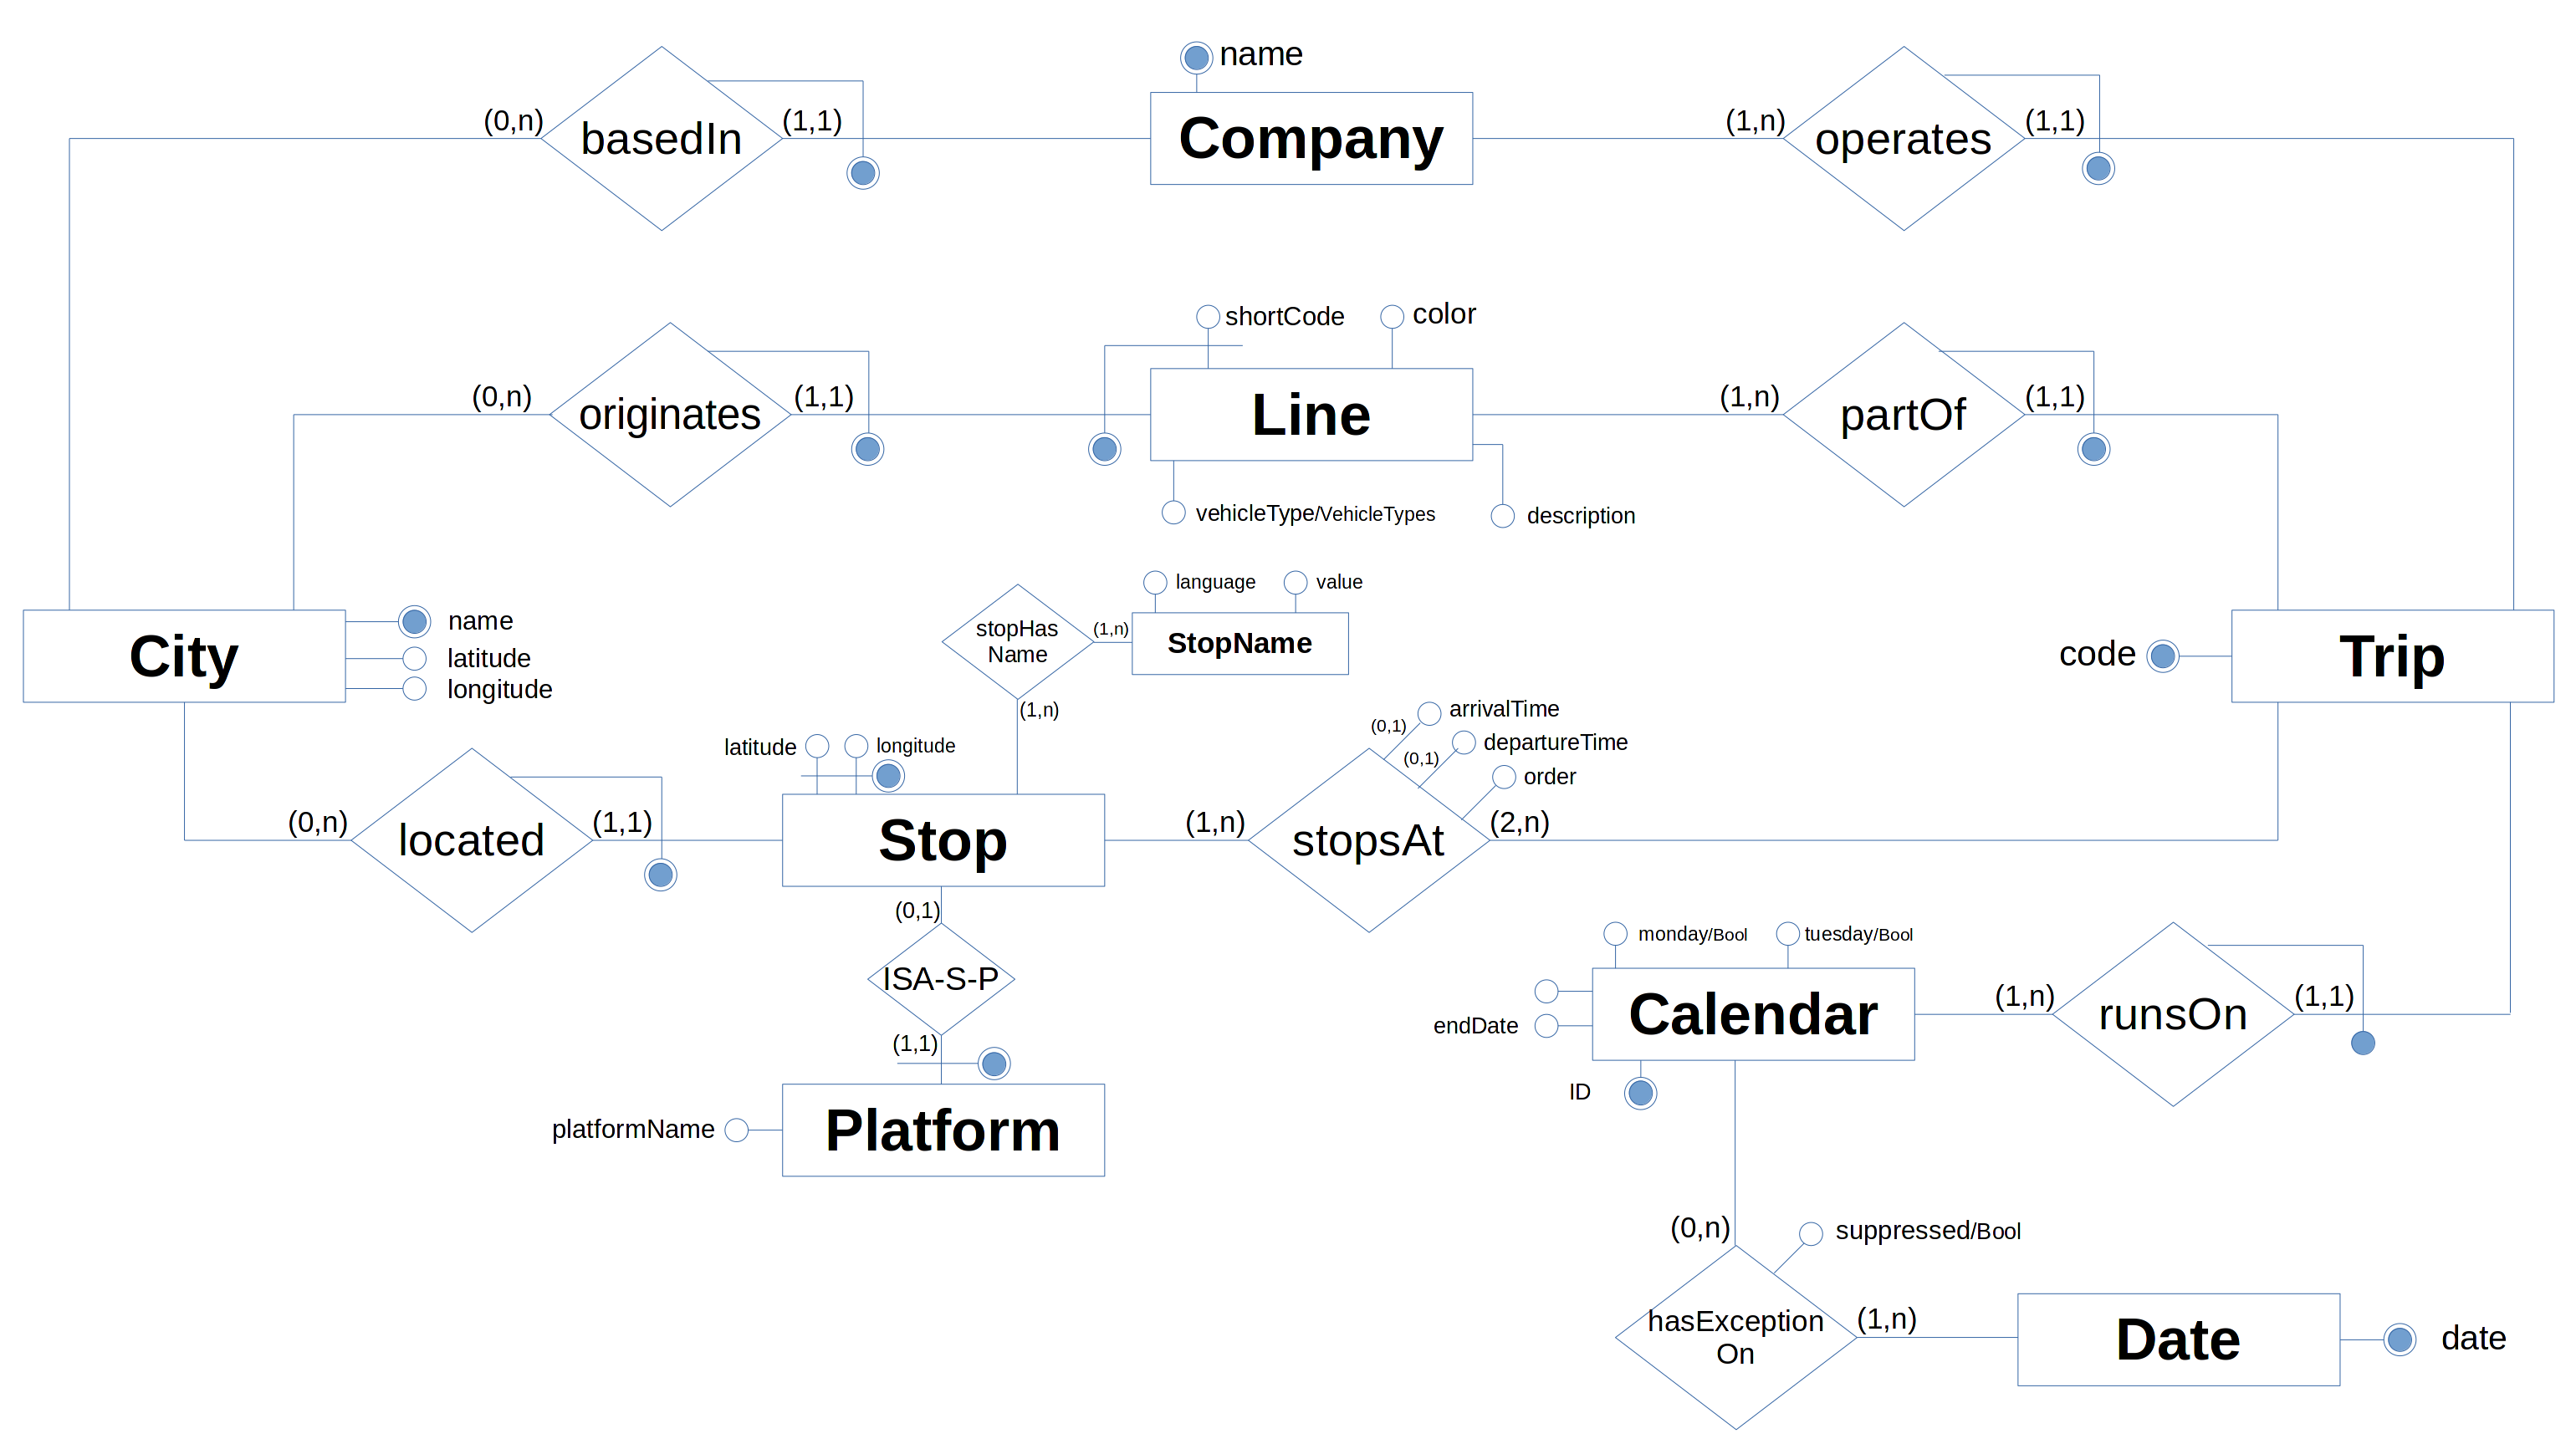
\includegraphics[height=\textheight]{diagram_rest}
		\caption{Restructured ER Schema \\ {\footnotesize \textit{Note: not all attributes have been indicated in the schema. Please check the \hyperref[sec:dictionary-rest]{data dictionary} for a complete overview}}}\label{img:diagram_rest}
	\end{figure}
\end{landscape}

\subsection{Reformulated Application Load}

	The following data is based on the original \hyperref[tbl:volumes]{table of volumes} and on the \hyperref[sec:assumptions]{assumptions}, particularly on point 4 about the translations. Regarding access tables, costs were written by considering the worst possible scenario (i.e. the one with maximal computational expense).

	\subsubsection{Table of Volumes}
	
	\begin{table}[h]
		\centering
		\begin{tabular}{|c|c|c|}
			\hline
			\textbf{Concept} & \textbf{Construct} & \textbf{Volume} \\
			\hline
			City & Entity & 30 \\ \hline
			Stop & Entity & 75 \\ \hline
			StopName & Entity & 150 \\ \hline
			Platform & Entity & 20 \\ \hline
			Trip & Entity & 500 \\ \hline
			Company & Entity & 5 \\ \hline
			Line & Entity & 25 \\ \hline
			Calendar & Entity & 10 \\ \hline
			Date & Entity & 200 \\ \hline
			basedIn & Relationship & 5 \\ \hline
			operates & Relationship & 500 \\ \hline
			originates & Relationship & 25 \\ \hline
			partOf & Relationship & 500 \\ \hline
			located & Relationship & 100 \\ \hline
			stopsAt & Relationship & 4500 \\ \hline
			runsOn & Relationship & 500 \\ \hline
			hasExceptionOn & Relationship & 150 \\ \hline
			stopHasName & Relationship & 150 \\ \hline
			ISA-S-P & Relationship & 30 \\ \hline
		\end{tabular}
		\caption{Restructured Table of Volumes}\label{tbl:volumes-rest}
	\end{table}

	\newpage
	\subsubsection{Access Tables}
	
	\paragraph{(1)} Get a list of \textit{(maximum)} ten stops with name in a specific language matching the user-given string
	
	\begin{table}[h!]
		\centering
		\begin{tabular}{|c|c|c|c|}
			\hline
			\textbf{Concept} & \textbf{Construct} & \textbf{Accesses} & \textbf{Type} \\
			\hline
			StopName & Entity & 75 & Read \\ \hline
			stopHasName & Relationship & 10 & Read \\ \hline
			Stop & Entity & 10 & Read \\ \hline 
			ISA-S-P & Relationship & 10 & Read \\ \hline
			Platform & Entity & 10 & Read \\ \hline
			located & Relationship & 10 & Read \\ \hline
			City & Entity & 10 & Read \\ \hline
		\end{tabular}
		\caption{Access table for operation 1}\label{tbl:access-1}
	\end{table}

	\paragraph{(2)} Get a list of \textit{(maximum)} ten stops with name in a specific language that are contained in a set of coordinates
	
	\begin{table}[h!]
		\centering
		\begin{tabular}{|c|c|c|c|}
			\hline
			\textbf{Concept} & \textbf{Construct} & \textbf{Accesses} & \textbf{Type} \\
			\hline
			Stop & Entity & 75 & Read \\ \hline 
			stopHasName & Relationship & 10 & Read \\ \hline
			StopName & Entity & 10 & Read \\ \hline
			located & Relationship & 10 & Read \\ \hline
			City & Entity & 10 & Read \\ \hline
			ISA-S-P & Relationship & 10 & Read \\ \hline
			Platform & Entity & 10 & Read \\ \hline
		\end{tabular}
		\caption{Access table for operation 2}\label{tbl:access-2}
	\end{table}

	\newpage
	\paragraph{(3)} Find the next ten trips, with line and company information, that depart from a specific stop at a given date and time \textit{(assuming that the stop coordinates are known)}

	\begin{table}[h!]
		\centering
		\begin{tabular}{|c|c|c|c|}
			\hline
			\textbf{Concept} & \textbf{Construct} & \textbf{Accesses} & \textbf{Type} \\
			\hline
			stopsAt & Relationship & 15 & Read \\ \hline
			Trip & Entity & 15 & Read \\ \hline
			runsOn & Relationship & 15 & Read \\ \hline
			Calendar & Entity & 15 & Read \\ \hline
			hasExceptionOn & Relationship & 225 & Read \\ \hline
			Date & Relationship & 225 & Read \\ \hline
			partOf & Relationship & 10 & Read \\ \hline
			Line & Entity & 10 & Read \\ \hline
			operates & Relationship & 10 & Read \\ \hline
			Company & Entity & 10 & Read \\ \hline
		\end{tabular}
		\caption{Access table for operation 3}\label{tbl:access-3}
	\end{table}

	\paragraph{(4)} Find the next ten trips departing from one stop and arriving at another one, at a given date and time \textit{(assuming that the stop coordinates are known)}
 
	\begin{table}[h!]
		\centering
		\begin{tabular}{|c|c|c|c|}
			\hline
			\textbf{Concept} & \textbf{Construct} & \textbf{Accesses} & \textbf{Type} \\
			\hline
			stopsAt & Relationship & 30 & Read \\ \hline
			Trip & Entity & 30 & Read \\ \hline
			runsOn & Relationship & 30 & Read \\ \hline
			Calendar & Entity & 30 & Read \\ \hline
			hasExceptionOn & Relationship & 225 & Read \\ \hline
			Date & Relationship & 225 & Read \\ \hline
			partOf & Relationship & 10 & Read \\ \hline
			Line & Entity & 10 & Read \\ \hline
			operates & Relationship & 10 & Read \\ \hline
			Company & Entity & 10 & Read \\ \hline
		\end{tabular}
		\caption{Access table for operation 4}\label{tbl:access-4}
	\end{table}

	\newpage
	\paragraph{(5)} Add a new company given the name and the headquarter city, \textit{and considering that all possible cities are already loaded into the database}
	
	\begin{table}[h!]
		\centering
		\begin{tabular}{|c|c|c|c|}
			\hline
			\textbf{Concept} & \textbf{Construct} & \textbf{Accesses} & \textbf{Type} \\
			\hline
			City & Entity & 1 & Read \\ \hline
			Company & Entity & 1 & Write \\ \hline 
			basedIn & Relationship & 1 & Write \\ \hline
		\end{tabular}
		\caption{Access table for operation 5}\label{tbl:access-5}
	\end{table}

	\paragraph{(6)} Add a new line given short code, color, type of vehicle and city, \textit{and considering that all possible cities are already loaded into the database}
	\begin{table}[h]
		\centering
		\begin{tabular}{|c|c|c|c|}
			\hline
			\textbf{Concept} & \textbf{Construct} & \textbf{Accesses} & \textbf{Type} \\
			\hline
			City & Entity & 1 & Read \\ \hline
			Line & Entity & 1 & Write \\ \hline
			originates & Relationship & 1 & Write \\ \hline
		\end{tabular}
		\caption{Access table for operation 6}\label{tbl:access-6}
	\end{table}

	\paragraph{(7)} Add a new trip given the code, the timetable, the operating company and the calendar
	\begin{table}[h]
		\centering
		\begin{tabular}{|c|c|c|c|}
			\hline
			\textbf{Concept} & \textbf{Construct} & \textbf{Accesses} & \textbf{Type} \\
			\hline
			Trip & Entity & 1 & Write \\ \hline
			stopsAt & Relationship & 9 & Write \\ \hline
			partOf & Relationship & 1 & Write \\ \hline
			operates & Relationship & 1 & Write \\ \hline
			runsOn & Relationship & 1 & Read \\ \hline
		\end{tabular}
		\caption{Access table for operation 7}\label{tbl:access-7}
	\end{table}

	\paragraph{(8)} Modify the schedule for a calendar knowing its code (add one exceptional date)
	\begin{table}[h!]
		\centering
		\begin{tabular}{|c|c|c|c|}
			\hline
			\textbf{Concept} & \textbf{Construct} & \textbf{Accesses} & \textbf{Type} \\
			\hline
			hasException & Relationship & 1 & Write \\ \hline
			Date & Entity & 1 & Write \\ \hline
		\end{tabular}
		\caption{Access table for operation 8}\label{tbl:access-8}
	\end{table}
	\section{Direct Translation}

\subsection{Relational schema}

	City(\uline{name}, latitude, longitude) \\
	
	
	Company(\uline{name})
	
	$ \ \ $ Inclusion: Company[name] $\subseteq$ Operates[company]
	
	$ \ \ $ Foreign Key: Company[name] $\subseteq$ BasedIn[company] \\
	
	
	Line(\uline{shortCode, cityName}, color, vehicleType, description)
	
	$ \ \ $ Foreign Key: Line[cityName] $\subseteq$ City[name]
	
	$ \ \ $ Inclusion: Line[shortCode, cityName] $\subseteq$ PartOf[lineCode, lineCity] \\

	
	Trip(\uline{code})
	
	$ \ \ $ Inclusion: Trip[code] $\subseteq$ StopsAt[trip]
	
	$ \ \ $ Foreign Key: Trip[code] $\subseteq$ PartOf[trip]
	
	$ \ \ $ Foreign Key: Trip[code] $\subseteq$ Operates[trip]
	
	$ \ \ $ Foreign Key: Trip[code] $\subseteq$ RunsOn[trip] \\
	
	
	Calendar(\uline{ID}, startDate, endDate, {\small monday, tuesday, wednesday, thurdsay, friday, saturday, sunday) }
	
	$ \ \ $ Inclusion: Calendar[ID] $\subseteq$ RunsOn[calendar] \\
	
	
	Date(\uline{date})
	
	$ \ \ $ Inclusion: Date[date] $\subseteq$ HasExceptionOn[date] \\
	
	
	Stop(\uline{latitude, longitude})
	
	$ \ \ $ Inclusion: Stop[latitude, longitude] $\subseteq$ StopsAt[latitude, longitude] 
	
	$ \ \ $ Inclusion: Stop[latitude, longitude] $\subseteq$ StopHasName[latitude, longitude] 
	
	$ \ \ $ Foreign key: Stop[latitude, longitude] $\subseteq$ Located[stopLat, stopLon] \\
	
	
	StopName(\uline{language, value})
	
	$ \ \ $ Inclusion: StopName[language, value] $\subseteq$ StopHasName[language, value] \\
	
	
	Platform(\uline{latitude, longitude}, platformName)
	
	$ \ \ $ Foreign Key: Platform[latitude, longitude] $\subseteq$ Stop[latitude, longitude] \\
	
	
	StopsAt(\uline{latitude, longitude, trip}, order, arrivalTime*, departureTime*)
	
	$ \ \ $ Foreign Key: StopsAt[latitude, longitude] $\subseteq$ Stop[latitude, longitude]
	
	$ \ \ $ Foreign Key: StopsAt[trip] $\subseteq$ Trip[code] \\
	
	
	StopHasName(\uline{latitude, longitude, language, value})
	
	$ \ \ $ Foreign Key: StopHasName[latitude, longitude] $\subseteq$ Stop[latitude, longitude]
	
	$ \ \ $ Foreign Key: StopHasName[language, value] $\subseteq$ StopName[language, value] \\
	
	Located(\uline{stopLat, stopLon}, cityName) 
	
	$ \ \ $ Foreign Key: Located[stopLat, stopLon] $\subseteq$ Stop[latitude, longitude]
	
	$ \ \ $ Foreign Key: Located[cityName] $\subseteq$ City[name] \\
	
	\newpage
	RunsOn(\uline{trip, calendar})
	
	$ \ \ $ Foreign Key: RunsOn[trip] $\subseteq$ Trip[code]
	
	$ \ \ $ Inclusion: RunsOn[calendar] $\subseteq$ Calendar[ID] \\
	
	
	HasExceptionOn(\uline{date, calendar}, suppressed)
	
	$ \ \ $ Foreign Key: HasExceptionOn[date] $\subseteq$ Date[date]
	
	$ \ \ $ Foreign Key: HasExceptionOn[calendar] $\subseteq$ Calendar[ID] \\
	

	BasedIn(\uline{company}, city)
	
	$ \ \ $ Foreign Key: BasedIn[city] $\subseteq$ City[name]
	
	$ \ \ $ Foreign Key: BasedIn[company] $\subseteq$ Company[name] \\
	
	
	Operates(\uline{trip}, company)
	
	$ \ \ $ Foreign Key: Operates[trip] $\subseteq$ Trip[code]
	
	$ \ \ $ Foreign Key: Operates[company] $\subseteq$ Company[name] \\
	
	
	PartOf(\uline{trip}, lineCode, lineCity)
	
	$ \ \ $ Foreign Key: PartOf[trip] $\subseteq$ Trip[code]
	
	$ \ \ $ Foreign Key: PartOf[lineCode, lineCity] $\subseteq$ Line[shortCode, city]
	
	
\subsection{External Constraints}

	Constraint 7) was added. It is originated from the fact that a trip must have at least two stops, which was previously indicated in the conceptual schema with minimum cardinality equal to 2.
	
	\begin{enumerate}
		\item For each tuple in the entity \texttt{Calendar}, the attribute \textit{endDate} must encode a date strictly greater than \textit{startDate}.
		
		\item For each tuple in the relationship \texttt{stopsAt}, the attribute \textit{departureTime} must encode a time greater or equal than \textit{arrivalTime}.
		
		\item In the relationship \texttt{stopsAt}, for the first stop of a trip (with \textit{order=1}), the attribute \textit{arrivalTime} must be omitted and \textit{departureTime} must be specified. For the last stop (with maximal \textit{order}), the attribute \textit{arrivalTime} must be specified and \textit{departureTime} must be omitted. For all the other stops, both attributes must be present.
		
		\item In the relationship \texttt{stopsAt}, the attribute \textit{order} must be equal to \texttt{1} for the first stop of a trip, and should be incremented by one for subsequent stops.
		
		\item In the relationship \texttt{stopsAt}, for every pair of tuples \textit{T1} and \textit{T2} within the same trip, if \textit{T1[order] < T2[order]}, then \textit{T1[departureTime] < T2[arrivalTime]}
		
		\item For a \texttt{Trip}, the exceptional dates defined through the \texttt{hasExceptionOn} relationship must be in between \textit{startDate} and \textit{endDate} defined by the corresponding \texttt{Calendar} instance. Moreover, if \textit{suppressed=True} then the corresponding day of week in the \texttt{Calendar} instance has value \textit{True}. At the opposite, if \textit{suppressed=False} then the corresponding day of week in \texttt{Calendar} has value \textit{False};
		
		\item In the relation \texttt{StopsAt}, the minimum number of tuples having the same value for the \textit{trip} attribute is two.
	\end{enumerate} 

\newpage
\subsection{Application Load}
	
	\paragraph{(1)} Get a list of \textit{(maximum)} ten stops with name in a specific language matching the user-given string
	\begin{table}[h]
		\centering
		\begin{tabular}{|c|c|c|}
			\hline
			\textbf{Concept} & \textbf{Accesses} & \textbf{Type} \\
			\hline
			StopName & 75 & Read \\ \hline
			StopHasName & 10 & Read \\ \hline
			Stop & 10 & Read \\ \hline
			ISA-S-P & 10 & Read \\ \hline
			Platform & 10 & Read \\ \hline
			Located & 10 & Read \\ \hline
			City & 10 & Read \\ \hline
		\end{tabular}
		\caption{Access table for operation 1}\label{tbl:conc.access-1}
	\end{table}
	
	\paragraph{(2)} Get a list of \textit{(maximum)} ten stops with name in a specific language that are contained in a set of coordinates
	\begin{table}[h]
		\centering
		\begin{tabular}{|c|c|c|}
			\hline
			\textbf{Concept} & \textbf{Accesses} & \textbf{Type} \\
			\hline
			Stop & 75 & Read \\ \hline 
			StopHasName & 10 & Read \\ \hline
			StopName & 10 & Read \\ \hline
			Located & 10 & Read \\ \hline
			City & 10 & Read \\ \hline
			ISA-S-P & 10 & Read \\ \hline
			Platform & 10 & Read \\ \hline
		\end{tabular}
		\caption{Access table for operation 2}\label{tbl:conc.access-2}
	\end{table}
	
	\newpage
	\paragraph{(3)} Find the next ten trips, with line and company information, that depart from a specific stop at a given date and time \textit{(assuming that the stop coordinates are known)}
	\begin{table}[h]
		\centering
		\begin{tabular}{|c|c|c|}
			\hline
			\textbf{Concept} & \textbf{Accesses} & \textbf{Type} \\
			\hline
			StopsAt & 15 & Read \\ \hline
			Trip & 15 & Read \\ \hline
			RunsOn & 15 & Read \\ \hline
			Calendar & 15 & Read \\ \hline
			HasExceptionOn & 225 & Read \\ \hline
			Date & 225 & Read \\ \hline
			PartOf & 10 & Read \\ \hline
			Line & 10 & Read \\ \hline
			Operates & 10 & Read \\ \hline
			Company & 10 & Read \\ \hline
		\end{tabular}
		\caption{Access table for operation 3}\label{tbl:conc.access-3}
	\end{table}
	
	\paragraph{(4)} Find the next ten trips departing from one stop and arriving at another one, at a given date and time \textit{(assuming that the stop coordinates are known)}
	
	\begin{table}[h]
		\centering
		\begin{tabular}{|c|c|c|}
			\hline
			\textbf{Concept} & \textbf{Accesses} & \textbf{Type} \\
			\hline
			StopsAt & 30 & Read \\ \hline
			Trip & 30 & Read \\ \hline
			RunsOn & 30 & Read \\ \hline
			Calendar & 30 & Read \\ \hline
			HasExceptionOn & 225 & Read \\ \hline
			Date & 225 & Read \\ \hline
			PartOf & 10 & Read \\ \hline
			Line & 10 & Read \\ \hline
			Operates & 10 & Read \\ \hline
			Company & 10 & Read \\ \hline
		\end{tabular}
		\caption{Access table for operation 4}\label{tbl:conc.access-4}
	\end{table}
	
	\newpage
	\paragraph{(5)} Add a new company given the name and the headquarter city, \textit{and considering that all possible cities are already loaded into the database}
	
	\begin{table}[h]
		\centering
		\begin{tabular}{|c|c|c|}
			\hline
			\textbf{Concept} & \textbf{Accesses} & \textbf{Type} \\
			\hline
			City & 1 & Read \\ \hline
			Company & 1 & Write \\ \hline 
			basedIn & 1 & Write \\ \hline
		\end{tabular}
		\caption{Access table for operation 5}\label{tbl:conc.access-5}
	\end{table}
	
	\paragraph{(6)} Add a new line given short code, color, type of vehicle and city, \textit{and considering that all possible cities are already loaded into the database}
	\begin{table}[h]
		\centering
		\begin{tabular}{|c|c|c|}
			\hline
			\textbf{Concept} & \textbf{Accesses} & \textbf{Type} \\
			\hline
			City & 1 & Read \\ \hline
			Line & 1 & Write \\ \hline
			originates & 1 & Write \\ \hline
		\end{tabular}
		\caption{Access table for operation 6}\label{tbl:conc.access-6}
	\end{table}
	
	\paragraph{(7)} Add a new trip given the code, the timetable, the operating company and the calendar
	\begin{table}[h]
		\centering
		\begin{tabular}{|c|c|c|}
			\hline
			\textbf{Concept} & \textbf{Accesses} & \textbf{Type} \\
			\hline
			Trip & 1 & Write \\ \hline
			stopsAt & 9 & Write \\ \hline
			partOf & 1 & Write \\ \hline
			Operates & 1 & Write \\ \hline
			RunsOn & 1 & Read \\ \hline
		\end{tabular}
		\caption{Access table for operation 7}\label{tbl:conc.access-7}
	\end{table}
	
	\paragraph{(8)} Modify the schedule for a calendar knowing its code (add one exceptional date)
	\begin{table}[h!]
		\centering
		\begin{tabular}{|c|c|c|}
			\hline
			\textbf{Concept} & \textbf{Accesses} & \textbf{Type} \\
			\hline
			HasException & 1 & Write \\ \hline
			Date & 1 & Write \\ \hline
		\end{tabular}
		\caption{Access table for operation 8}\label{tbl:conc.access-8}
	\end{table}
	\section{Restructuring of the relational schema}

\noindent The obtained relational schema can be further optimized.

\medskip
Firstly, some redundant relations are found: \texttt{StopName} and \texttt{HasName}, and also \texttt{Date} and \texttt{HasExceptionOn}. In both cases, one may see that the first relations consist of just one attribute, and that the same attribute is already included in the second relations as a foreign key. It is therefore reasonable to delete \texttt{StopName} and \texttt{Date}, because the relevant data can be queried by using the \texttt{HasName} and \texttt{HasExceptionOn}.

\medskip
In general, it was noticed that the complexity of queries for interactive operations (i.e. 1-4) was quite high and it involved a considerable number of joins between relations. For this reason, the decision taken was to delete those relations deriving from relationships in the original schema, where one role had cardinality \textit{(1,1)}, for example \textit{RunsOn, PartOf, ...}. These relations have been merged into the role with cardinality \textit{(1,1)}; the inclusion, foreign key and external constraints have been modified accordingly.

\medskip
Another context in which a relation may be deleted is the one of \texttt{Stop} and \texttt{Platform}. The latter relation contains the name of the platform, plus a reference to the Stop relation. To reduce the number of joins needed to perform the various operations, it has been chosen to merge those relations together. The \texttt{Stop} relation will then gain a new \textit{nullable} attribute, \texttt{platformName}. Even though this increases the number of pages in the relation, it is also reducing the queries complexity, in particular the one of operations 3 and 4. Since those operations are interactive, more importance has been given to execution time rather than space efficiency.

\subsection{Restructured schema}

	City(\uline{name}, latitude, longitude) \\


	Company(\uline{name}, headquarterCity)

	$ \ \ $ Foreign key: Company[headquarterCity] $\subseteq$ City[name] \\


	Line(\uline{shortCode, departingCity}, color, vehicleType, description)

	$ \ \ $ Foreign Key: Line[departingCity] $\subseteq$ City[name]

	$ \ \ $ Inclusion: Line[shortCode, departingCity] $\subseteq$ Trip[lineCode, lineCity] \\


	Trip(\uline{code}, calendar, company, lineCode, lineCity)

	$ \ \ $ Inclusion: Trip[code] $\subseteq$ StopsAt[trip]

	$ \ \ $ Foreign Key: Trip[calendar] $\subseteq$ Calendar[ID]

	$ \ \ $ Foreign Key: Trip[company] $\subseteq$ Company[name]

	$ \ \ $ Foreign Key: Trip[lineCode,lineCity] $\subseteq$ Line[shortCode,departingCity] \\


	Calendar(\uline{ID}, startDate, endDate, {\small monday, tuesday, wednesday, thurdsay, friday, saturday, sunday) }

	$ \ \ $ Inclusion: Calendar[ID] $\subseteq$ Trip[calendar] \\


	Stop(\uline{latitude, longitude}, city, platformName*)

	$ \ \ $ Inclusion: Stop[latitude, longitude] $\subseteq$ StopsAt[latitude, longitude]

	$ \ \ $ Inclusion: Stop[latitude, longitude] $\subseteq$ StopHasName[latitude, longitude]

	$ \ \ $ Foreign Key: Stop[city] $\subseteq$ City[name] \\

	\newpage
	StopsAt(\uline{latitude, longitude, trip}, order, arrivalTime*, departureTime*)

	$ \ \ $ Foreign Key: StopsAt[latitude, longitude] $\subseteq$ Stop[latitude, longitude]

	$ \ \ $ Foreign Key: StopsAt[trip] $\subseteq$ Trip[code] \\


	StopHasName(\uline{latitude, longitude, language} value)

	$ \ \ $ Foreign Key: StopHasName[latitude, longitude] $\subseteq$ Stop[latitude, longitude] \\


	HasExceptionOn(\uline{date, calendar}, suppressed)

	$ \ \ $ Foreign Key: HasExceptionOn[calendar] $\subseteq$ Calendar[ID]

\subsection{External Constraints}

\begin{enumerate}
	\item For each tuple in the entity \texttt{Calendar}, the attribute \textit{endDate} must encode a date strictly greater than \textit{startDate}.

	\item For each tuple in the relationship \texttt{stopsAt}, the attribute \textit{departureTime} must encode a time greater or equal than \textit{arrivalTime}.

	\item In the relationship \texttt{stopsAt}, for the first stop of a trip (with \textit{order=1}), the attribute \textit{arrivalTime} must be omitted and \textit{departureTime} must be specified. For the last stop (with maximal \textit{order}), the attribute \textit{arrivalTime} must be specified and \textit{departureTime} must be omitted. For all the other stops, both attributes must be present.

	\item In the relationship \texttt{stopsAt}, the attribute \textit{order} must be equal to \texttt{1} for the first stop of a trip, and should be incremented by one for subsequent stops.

	\item In the relationship \texttt{stopsAt}, for every pair of tuples \textit{T1} and \textit{T2} within the same trip, if \textit{T1[order] < T2[order]}, then \textit{T1[departureTime] < T2[arrivalTime]}

	\item For a \texttt{Trip}, the exceptional dates defined through the \texttt{hasExceptionOn} relationship must be in between \textit{startDate} and \textit{endDate} defined by the corresponding \texttt{Calendar} instance. Moreover, if \textit{suppressed=True} then the corresponding day of week in the \texttt{Calendar} instance has value \textit{True}. At the opposite, if \textit{suppressed=False} then the corresponding day of week in \texttt{Calendar} has value \textit{False};

	\item In the relation \texttt{StopsAt}, the minimum number of tuples having the same value for the \textit{trip} attribute is two.
\end{enumerate}

\newpage
\subsection{Application Load}

\paragraph{(1)} Get a list of \textit{(maximum)} ten stops with name in a specific language matching the user-given string

\begin{table}[h]
	\centering
	\begin{tabular}{|c|c|c|}
		\hline
		\textbf{Concept} & \textbf{Accesses} & \textbf{Type} \\
		\hline
		StopHasName & 75 & Read \\ \hline
		Stop & 10 & Read \\ \hline
	\end{tabular}
	\caption{Access table for operation 1}\label{tbl:rest.access-1}
\end{table}

\paragraph{(2)} Get a list of \textit{(maximum)} ten stops with name in a specific language that are contained in a set of coordinates

\begin{table}[h]
	\centering
	\begin{tabular}{|c|c|c|}
		\hline
		\textbf{Concept} & \textbf{Accesses} & \textbf{Type} \\
		\hline
		Stop & 75 & Read \\ \hline
		StopHasName & 10 & Read \\ \hline
	\end{tabular}
	\caption{Access table for operation 2}\label{tbl:rest.access-2}
\end{table}

\paragraph{(3)} Find the next ten trips, with line and company information, that depart from a specific stop at a given date and time \textit{(assuming that the stop coordinates are known)}
\begin{table}[h]
	\centering
	\begin{tabular}{|c|c|c|}
		\hline
		\textbf{Concept} & \textbf{Accesses} & \textbf{Type} \\
		\hline
		StopsAt & 15 & Read \\ \hline
		Trip & 15 & Read \\ \hline
		Calendar & 15 & Read \\ \hline
		HasExceptionOn & 225 & Read \\ \hline
		Line & 10 & Read \\ \hline
	\end{tabular}
	\caption{Access table for operation 3}\label{tbl:rest.access-3}
\end{table}

\paragraph{(4)} Find the next ten trips departing from one stop and arriving at another one, at a given date and time \textit{(assuming that the stop coordinates are known)}
\begin{table}[h!]
	\centering
	\begin{tabular}{|c|c|c|}
		\hline
		\textbf{Concept} & \textbf{Accesses} & \textbf{Type} \\
		\hline
		StopsAt & 30 & Read \\ \hline
		Trip & 30 & Read \\ \hline
		Calendar & 30 & Read \\ \hline
		HasExceptionOn & 225 & Read \\ \hline
		Line & 10 & Read \\ \hline
	\end{tabular}
	\caption{Access table for operation 4}\label{tbl:rest.access-4}
\end{table}

\paragraph{(5)} Add a new company given the name and the headquarter city, \textit{and considering that all possible cities are already loaded into the database}

\begin{table}[h]
	\centering
	\begin{tabular}{|c|c|c|}
		\hline
		\textbf{Concept} & \textbf{Accesses} & \textbf{Type} \\
		\hline
		City & 1 & Read \\ \hline
		Company & 1 & Write \\ \hline
	\end{tabular}
	\caption{Access table for operation 5}\label{tbl:rest.access-5}
\end{table}

\paragraph{(6)} Add a new line given short code, color, type of vehicle and city, \textit{and considering that all possible cities are already loaded into the database}

\begin{table}[h]
	\centering
	\begin{tabular}{|c|c|c|}
		\hline
		\textbf{Concept} & \textbf{Accesses} & \textbf{Type} \\
		\hline
		City & 1 & Read \\ \hline
		Line & 1 & Write \\ \hline
	\end{tabular}
	\caption{Access table for operation 6}\label{tbl:rest.access-6}
\end{table}

\paragraph{(7)} Add a new trip given the code, the timetable, the operating company and the calendar

\begin{table}[h]
	\centering
	\begin{tabular}{|c|c|c|}
		\hline
		\textbf{Concept} & \textbf{Accesses} & \textbf{Type} \\
		\hline
		Trip & 1 & Write \\ \hline
		stopsAt & 9 & Write \\ \hline
	\end{tabular}
	\caption{Access table for operation 7}\label{tbl:rest.access-7}
\end{table}

\paragraph{(8)} Modify the schedule for a calendar knowing its code (add one exceptional date)
\begin{table}[h!]
	\centering
	\begin{tabular}{|c|c|c|}
		\hline
		\textbf{Concept} & \textbf{Accesses} & \textbf{Type} \\
		\hline
		HasException & 1 & Write \\ \hline
	\end{tabular}
	\caption{Access table for operation 8}\label{tbl:rest.access-8}
\end{table}

\section{SQL Specification}

	Three attatched files are present in the \texttt{sql} directory:
	\begin{itemize}[itemsep=0pt]
		\item \texttt{base.sql} contains the definition of the various relations
		\item \texttt{data.sql} contains some sample data
		\item \texttt{full.sql} is the dump of the complete database, left for fallback
	\end{itemize}

	They may be imported into a local instance with the following commands:
	\begin{center}
		\begin{lstlisting}
			psql
			postgres=# \i base.sql
			publictransport_17573=# \i data.sql
		\end{lstlisting}
	\end{center}

	As it may be seen, tuple and external constraints have been implemented either as CHECK operations or as triggers with stored procedures. Note that external constraints 5-6 were considered too difficult and as such they have not been implemented. Constraint 4 was implemented by relying on postgres' \texttt{Serial} data type, which represents an increasing integer that start from 1. The domain \texttt{VehicleType} for a \textit{Line} has been created as a custom type.

\subsection{Queries related to the operations}

	\paragraph{(1)} Get a list of \textit{(maximum)} ten stops with name in a specific language matching the user-given string. \textit{Parameters: stop name, language}
	\begin{center}
		\begin{lstlisting}
	SELECT S.city, SN.value AS name, S.latitude, S.longitude
	FROM Stop S, StopHasName SN
	WHERE S.latitude=SN.latitude AND S.longitude=SN.longitude
	AND SN.value ILIKE _name_ AND SN.language=_language_;
		\end{lstlisting}
	\end{center}

	\paragraph{(2)} Get a list of \textit{(maximum)} ten stops with name in a specific language that are contained in a set of coordinates. \textit{Parameters: latitude, longitude, radius, language}
	\begin{center}
	\begin{lstlisting}
	SELECT S.city, SN.value AS name, S.latitude, S.longitude
	FROM Stop S, StopHasName SN
	WHERE SN.latitude=S.latitude AND SN.longitude=S.longitude
	AND acos( cos(radians(_latitude_)) * cos(radians(S.latitude)) *
	cos(radians(S.longitude) - radians(_longitude_)) + sin(radians(_latitude_)) *
	sin(radians(S.latitude)) ) * 6371393 <= _radius_
	AND S.platformName IS NULL AND SN.language=_language_;
	\end{lstlisting}
\end{center}

	\newpage
	\paragraph{(3)} Find the next ten trips, with line and company information, that depart from a specific stop at a given date and time. \textit{Parameters: stop latitude, stop longitude, date and time}
	\begin{center}
		\begin{lstlisting}
	SELECT T.company, L.shortCode AS Line, L.vehicleType, T.code as "Trip Code",
	  SA.departureTime AS "Departure Time"
	FROM trip T, calendar C, stopsAt SA, line L
	WHERE SA.latitude=_stopLat_ AND SA.longitude=_stopLon
	AND SA.departureTime>=_time_ AND T.calendar=C.ID
	AND T.code=SA.trip AND T.lineCode=L.shortCode
	AND (
	((C._dayOfWeek_=True) AND (_date_ NOT IN (SELECT date FROM HasExceptionOn E
		WHERE suppressed=True AND E.calendar=C.ID)))
	OR (_date_ IN (SELECT date FROM HasExceptionOn E
		WHERE suppressed=False AND E.calendar=C.ID))
	)
	ORDER BY SA.arrivalTime
	LIMIT 10;
		\end{lstlisting}
	\end{center}

	\paragraph{(4)} Find the next ten trips departing from one stop and arriving at another one, at a given date and time. \textit{Parameters: latitude and longitude for the two stops, date and time}
	\begin{center}
		\begin{lstlisting}
	SELECT T.company, L.shortCode AS Line, L.vehicleType, T.code as "Trip Code",
	  S1.departureTime AS "Departure Time", S2.arrivalTime AS "Arrival Time",
	  (S2.arrivalTime-S1.departureTime) AS duration
	FROM trip T, calendar C, stopsAt S1, stopsAt S2, line L
	WHERE S1.latitude=_s1lat_ AND S1.longitude=_s1lat_ AND S2.latitude=_s2lat_
	AND S2.longitude=_s2lon_ AND S1.departureTime>=_time_
	AND S1.trip=S2.trip AND T.calendar=C.ID AND T.code=S1.trip
	AND T.lineCode=L.shortCode
	AND (
	((C._dayOfWeek_=True) AND (_date_ NOT IN (SELECT date FROM HasExceptionOn E
		WHERE suppressed=True AND E.calendar=C.ID)))
	OR (_date_ IN (SELECT date FROM HasExceptionOn E
		WHERE suppressed=False AND E.calendar=C.ID))
	)
	ORDER BY S1.arrivalTime
	LIMIT 10;
		\end{lstlisting}
	\end{center}

	\paragraph{(5)} Add a new company given the name and the headquarter city. \textit{Parameters: company name, company city}
	\begin{center}
		\begin{lstlisting}
		INSERT INTO Company(name,headquarterCity) VALUES(...);
		\end{lstlisting}
	\end{center}

	\paragraph{(6)} Add a new line given short code, color, type of vehicle and city. \textit{Parameters: line short code, departing city, color, vehicle type}
	\begin{center}
		\begin{lstlisting}
	INSERT INTO Line(shortCode, color, vehicleType, cityName) VALUES (...);
		\end{lstlisting}
	\end{center}

	\paragraph{(7)} Add a new trip given the code, the timetable, the operating company and the calendar. \textit{Parameters: trip code, calendar ID, line code and departing city, company name. List of stops with the timetable (arrival and departure time)}
	\begin{center}
		\begin{lstlisting}
	INSERT INTO Trip(code,calendar,lineCode,lineCity,company) VALUES (...);
	INSERT INTO StopsAt(latitude,longitude,arrivalTime,departureTime) VALUES (...);
		\end{lstlisting}
	\end{center}

	\paragraph{(8)} Modify the schedule for a calendar knowing its code (add one exceptional date). \textit{Parameters: date, calendar ID, suppression state}
	\begin{center}
		\begin{lstlisting}
	INSERT INTO HasExceptionOn(date, calendar, suppressed) VALUES (...);
		\end{lstlisting}
	\end{center}

\section{Java Applcation}

	The Java code is available in the \texttt{app/code.zip }file. A ready-to-be-run file is found in the \texttt{app} directory. It may be executed in a terminal with:
	\begin{center}
		\begin{lstlisting}
		java -jar app/publictransport_17573.jar
		\end{lstlisting}
	\end{center}

	Note that Java 15 is required. It may be needed to specify the path to postgresql driver with \texttt{-classpath} argument. The connection parameters may be altered by modifying the \texttt{database.properties} file.

	The application allows to execute the queries related to the table of operations. After the initialization, the user is presented with a menu, from which all operations can be run:

	\begin{center}
		\centering
		\begin{lstlisting}
		****** Introduction to Databases project ******

		Connecting... successfully connected to the database


		------------ MENU ------------
		1) Stops by name
		2) Stops by coordinates
		3) Trips per Stop
		4) Trips between two stops
		5) Add new company
		6) Add new line
		7) Add new trip
		8) Modify calendar schedule
		9) Exit
		------------------------------
		Please choose an item:
		\end{lstlisting}
	\end{center}


\end{document}
